\section{Evaluation}
\label{sect:evaluation}

We have implemented a \sysname prototype as a Django web application
that features the REST API presented in Section~\ref{sect:fairtest}.
We evaluated our prototype by using it to uncover {\it privacy bugs}
in the pricing policy of the ``Staples Inc.'', as described by the
Wall Street Journal in 2012. We sought answer to the following three
questions:

\begin{enumerate}
  \item[{\bf Q1}] Can \sysname uncover {\em privacy bugs} for
    a pricing policy similar to the policy of the ``Staples Inc.''
    online store?
  \item[{\bf Q2}] What is the impact of {\em privacy bugs} in the outputs
    shown to users?
  \item[{\bf Q3}] What is impact of pricing policies on {\em privacy bugs}?
    Are {\em privacy bugs} inherent to any pricing policy, or are
    dependant on pricing policies?
\end{enumerate}

\subsection{\normalsize Methodology}
Our experimental evaluation of \sysname consists of the following three steps:

\begin{enumerate}
  \item
  Generate one million synthetic users that are spread across the
  areas corresponding to 40,000 US zip-codes. These synthetic users
  have four attributes: zip-code, race, sex, and income, and match
  the demographic characteristics of the US population, according to
  the US Census Bureau~\cite{CensusBureau}, as of May 3, 2014.
  \footnote{
    The infrastructure necessary for generating synthetic users is
    provided by a project of the ``Advanced Distributed Systems'' course,
    taught by professor Roxana Geambasu, Spring 2015. The developers of this
    project are Z. Zhou, Z. Wan, and X. Ma.
  }

  \item
  With the users generated in Step 1, simulate one million visits on
  an online store whose pricing policy is similar to the pricing policy
  of the ``Staples Inc.''.
  After each visit, register to \sysname the respective synthetic user
  along with the output received.

  \item
  Query \sysname's web interface to uncover any strong correlation between
  outputs and protected user attributes, i.e., race, income, and sex.
\end{enumerate}

Since user-attributes match the demographics of the US population,
race, sex, and income are assigned values that depend on zip-code. This is
because
the later defines the area in which a user lives in. In other words, user's race,
sex, and income correlate with user's zip-code, but not amongst each other.
Each synthetic user has
one of the following seven races: ``White'', ``Hispanic'', ``African
American'', ``Indian or Alaskan'', ``Asian'', ``Pacific Islander'', ``Other'',
and ``Two or More''. Also, each user is either ``Male'' or ``Female''. Finally,
each user has an income the lies into one of the following seven ranges:
``less then $\$5,000$'', ``more than $\$5,000$'', ``more than $\$10,000$'',
``more than $\$20,000$'', ``more than $\$40,000$'', ``more than $\$80,000$'',
``more than $\$160,000$'', ``more than $\$320,000$''.

\subsection{\normalsize Uncovering {\em Privacy Bugs}}
\label{sect:uncovering}
In this section we use \sysname to uncover potential {\em privacy bugs}
when one million synthetic users visit an online store which
implements the following pricing policy:
{\it if a user's distance from a competitor's store
(``OfficeDepot \& OfficeMax'') is less than 20 miles, show a low price;
otherwise, show a high price.} This pricing schema is similar to the pricing
policy implemented by the ``Staples Inc.'' online store, as of the Wall Street
Journal, 2012.

To evaluate the presence of {\em privacy bugs}, we measure the
value of the delta of {\em statistical parity}
(condition~\ref{eq:StatisticalParity} -
introduced in Section~\ref{sect:statparity})
We group users based on (a) income, (b) race, and (c) sex, and examine potential
violations of condition~\ref{eq:StatisticalParity} for $\epsilon=0.05$ and
output being ``high'' price. Figure~\ref{fig:Deltas} shows the deltas
for user's race, income, and sex, as a function of price engine's dependency
on user' s location. When price engine's dependency on user's location is zero,
all users receive random prices. When price engine's dependency on users
location is 100\%, all users receive prices strictly based on the rule
introduced in the previous paragraph.


Figure~\ref{fig:DeltasIncome} reveals that when users are grouped according to
their income, {\em statistical parity} is not dependant on user's location,
except for users with annual income ``more than \$320,000''. Users whose income
lie in the later categorie are treated differently (favorably or unfavorably)
than the rest, and their location correlates with the outputs (i.e., prices)
they receive. Also, Figure~\ref{fig:DeltasRace} indicates that when users are
grouped according to their race, {\em statistical parity} is not dependant on
user's location, unless the user is an Indian American or an Alaskan.
This signals that Indian Americans and Alaskans are treated differently
(favorably or unfavorably) than the rest.

Given the fact that both user's race and user's income are a protected
attribute, one can use \sysname's reports to conclude that the implemented
pricing policy imposes an undesirable privacy bug, which is
summarized as follows: ``If the user is an Indian American or an Alaskan, or
has an income more than \$320,000, he or she will consistently be treated
differently than others.''
On the other hand, Figure~\ref{fig:DeltasSex} indicates when users are grouped
according to their sex, {\em statistical parity} is independent of user's
location, and therefore males are treated similarly to females.

\begin{figure*}[t]
{
  \subfigure[Income]{
    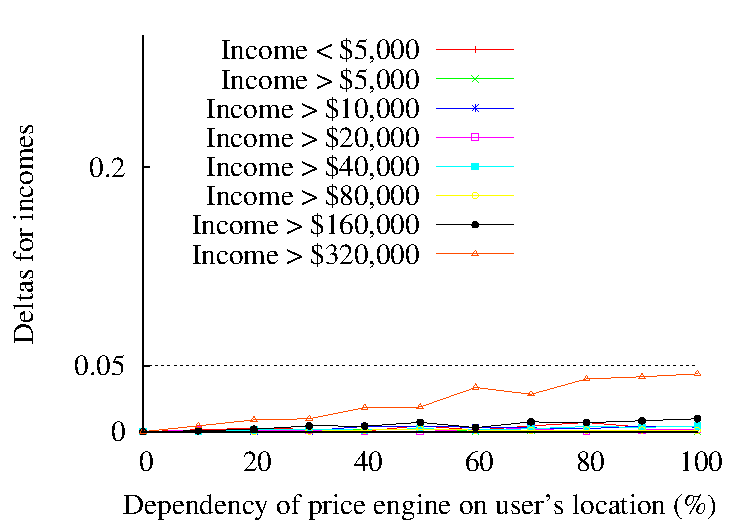
\includegraphics[width=0.33\textwidth]
    {\detokenize{results/income_discrimination_on_location_dependency}}
    \label{fig:DeltasIncome}
  }
  \subfigure[Race]{
    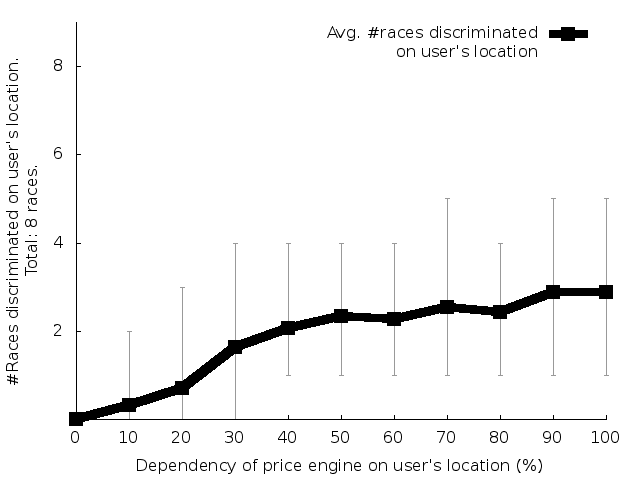
\includegraphics[width=0.33\textwidth]
    {\detokenize{results/race_discrimination_on_location_dependency}}
    \label{fig:DeltasRace}
  }
  \subfigure[Sex]{
    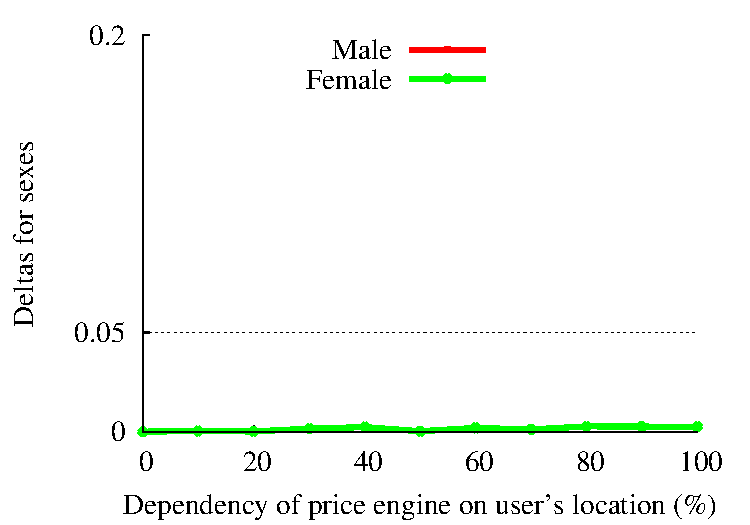
\includegraphics[width=0.33\textwidth]
    {\detokenize{results/sex_discrimination_on_location_dependency}}
    \label{fig:DeltasSex}
  }
  \caption{\textbf{Statistical parity and its dependency on user's location.}
          Shows the dependency of statistical parity on user's location,
          when users are grouped based on (a) income, (b) race, and (c) sex.
          Figures (a) and (b) reveal that when users are grouped according to
          income and race, statistical parity correlates for some groups with
          the dependency of the price engine on user's location. While Figure
          (c) reveals that statistical parity is independent of user's location
          when users are grouped based on sex.
  }
  \label{fig:Deltas}
}
\end{figure*}

\begin{figure*}[t]
{
  \subfigure[Income]{
    \includegraphics[width=0.33\textwidth]
    {\detokenize{results/income_discrimination_on_proportional}}
    \label{fig:IncomeDiscriminationProportional}
  }
  \subfigure[Race]{
    \includegraphics[width=0.33\textwidth]
    {\detokenize{results/race_discrimination_on_proportional}}
    \label{fig:RaceDiscriminationProportional}
  }
  \subfigure[Sex]{
    \includegraphics[width=0.33\textwidth]
    {\detokenize{results/sex_discrimination_on_proportional}}
    \label{fig:SexDiscriminationProportional}
  }
  \caption{\textbf{Prices shown to users and their dependency on income,
          race, and sex.} Shows the proportion of high versus low
          prices shown to users based on (a) income, (b) race, and (c) sex.
          Figure (a) reveals that a user with annual income less than
          \$5,000 receives proportionaly more high prices than a user with
          annual income more than \$320,000. Figure (b) indicates that an
          Indian American or an Alaskan users receives notably more high prices
          than any other user. This raises a consern, since as shown in
          Figure~\ref{fig:IncomePerRace}, an Indian American or an Alaskan
          user has on average a considerably lower annual income than a
          white American user. Figure (c) shows that male and female users
          receive approximately the same proportion of high versus
          low prices.
  }
  \label{fig:DiscriminationProportional}
}
\end{figure*}
\begin{figure}[t]
 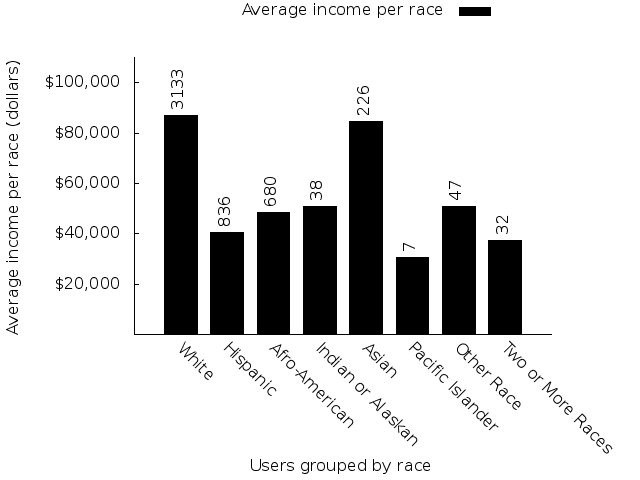
\includegraphics[width=0.49\textwidth]
  {\detokenize{results/income_per_race}}
  \caption{\textbf{Average annual income per race.} An Indian or an Alaskan user has
           a considerably lower income than a white American, and yet, as shown in
           Figure~\ref{fig:IncomeDiscriminationProportional}, he or she receives
           proportionally more high prices.
  }
  \label{fig:IncomePerRace}
\end{figure}

\subsection{\normalsize Measuring the Impact of {\em Privacy Bugs}}
Having concluded that the aforementioned pricing policy violates {\em statistical
parity} of users, i.e., introduces {\em privacy bugs}, we now investigate the
impact of these bugs. To this end, we examine whether users are treated
favorably or unfavorably by measuring the proportion of ``high'' versus ``low''
prices shown to users. Figure~\ref{fig:DiscriminationProportional} shows, in
percentage, the proportion of ``high'' versus ``low'' prices shown to them
grouped by user's (a) race, (b) income, and (c) sex. Also, on top of each bar the
raw number of members of the respective group is shown.

Figure~\ref{fig:IncomeDiscriminationProportional} shows that for each income
group, around 6\% of users receive ``high'' prices (the rest receive ``low''
prices), except the income group which includes users with annual income
``more than \$320,000''. Recall that based on Figure~\ref{fig:DeltasIncome}, we
had already concluded that users with annual income ``more than \$320,000'' are
treated differently that the rest. Additionally,
Figure~\ref{fig:IncomeDiscriminationProportional} helps conclude that users with
annual income ``more than \$320,000'' are treated favorably compare to the rest.
Note that a user with annual income ``less than \$5,000'' is more probable to
receive a high price, than a user with annual income ``more than \$320,000''.
Clearly this is a very poor -- yet unintentional -- algorithmic decision imposed
by a privacy bug which is difficult to foresee without the aid of \sysname.


Figure~\ref{fig:RaceDiscriminationProportional} helps conclude that the
percentage of ``high'' prices shown to ``Indian Americans and Alaskans'' is
notably higher than any other race. Recall that by analyzing
Figure~\ref{fig:DeltasRace}, we had already concluded that
``Indian Americans and Alaskans'' are treated differently than the rest.
In addition, Figure~\ref{fig:RaceDiscriminationProportional} reveals that
``Indian Americans and Alaskans'' are treated unfavorably, since they are
more probable to receive a ``high'' price, than the rest. This is also a very
poor algorithmic decision, because as shown in Figure~\ref{fig:IncomePerRace},
``Indian Americans and Alaskans'' have a low annual income on average. In
other words, the enforced pricing policy consistently shows more
``high'' prices to populations with lower annual income.
Although this is an unintentional effect of a reasonable algorithmic decision,
it may actually attract negative criticism. We believe that \sysname helps
increase developers' transparency on such kind of side effects, and minimize
the unpredictable danger of discriminatory treatment of populations.

\subsection{\normalsize Measuring the Impact of Pricing Policies}
Finally, we examine the impact of different pricing policies on the presence
of {\em privacy bugs}, and seek to understand how algorithmic decision
affect {\em privacy bugs}. To achieve this, we modify the pricing policy
to now abide by the following rule: {\it if a user's distance from a
competitor's store (``OfficeDepot \& OfficeMax'') is less than 10 miles,
show a low price; otherwise, show a high price.} Then, we compare the outputs
shown to users in this case, against the outputs shown to users with the policy
introduced in Section~\ref{sect:uncovering}. Note that the only modification 
is the change on user's distance from competitor's stores (from 20 miles
to 10 miles).

Figure~\ref{fig:DiscriminationProportionalAdditional} shows that after
applying the new  pricing policy more users receive ``high'' prices
compared to Figure~\ref{fig:DiscriminationProportional}. This is expected
since we apply a stricter policy that shows ``low'' if the competitor's
stores are within 10 miles,  instead of 20 miles. Notably, however, Indian Americans
and Alaskans are still the most unfavorably treated populations. Also, users
with annual income ``more than \$320,000'' are still the most favorably treated
population. This indicates that despite variations of the pricing policies,
there are inherent correlations between user attributes that are transparent
to developers, have it not been \sysname. Hence, we believe that \sysname
helps increase developers transparency on data use and provide some understanding
on: the policies applied on the data.


\subsection{\normalsize Summary of Results}
Overall, these result highlight the danger of discriminatory treatment of
users as a results of legitimate algorithmic decisions. Although developers
design policies to optimize for their needs, these policies have unpredictable
side effects on data, and may result into objectionable situations. With simulating
``Staples Inc.'' pricing policy, we show-cased how \sysname helps increase
developers' transparency on data use, uncover {\em privacy bugs}, and report
these bugs to developers.

\begin{figure*}[t]
{
 \subfigure[Income]{
    \includegraphics[width=0.33\textwidth]
    {\detokenize{results/misc/income_discrimination_on_proportional}}
    \label{fig:IncomeDiscriminationProportionalAdditional}
  }
  \subfigure[Race]{
    \includegraphics[width=0.33\textwidth]
    {\detokenize{results/misc/race_discrimination_on_proportional}}
    \label{fig:RaceDiscriminationProportionalAdditional}
  }
  \subfigure[Sex]{
    \includegraphics[width=0.33\textwidth]
    {\detokenize{results/misc/sex_discrimination_on_proportional}}
    \label{fig:SexDiscriminationProportionalAdditional}
  }
  \caption{\textbf{Prices shown to users and their dependency on income,
          race, and sex.} Shows the proportion of high versus low
          prices shown to users based on (a) income, (b) race, and (c) sex.
          In this case, the pricing policy is stricter and results to ``low''
          prices if user's distance from a competitor's store is less than 10
          miles. Figure (a) reveals that a users with annual income less than
          \$5,000 still receives proportionally more high prices than a user with
          annual income more than \$320,000. Figure (b) indicates that an
          Indian American or an Alaskan users still receives notably more high
          prices than any other user. Figure (c) shows that male and female
          users receive approximately the same proportion of high versus
          low prices.
  }
  \label{fig:DiscriminationProportionalAdditional}
}
\end{figure*}
